\documentclass[conference]{IEEEtran}
\IEEEoverridecommandlockouts
% The preceding line is only needed to identify funding in the first footnote. If that is unneeded, please comment it out.
%Template version as of 6/27/2024

\usepackage{cite}
\usepackage{amsmath,amssymb,amsfonts}
\usepackage{algorithmic}
\usepackage{graphicx}
\usepackage{textcomp}
\usepackage{xcolor}
\usepackage{booktabs}
\usepackage{multirow}
\usepackage{array}
\usepackage{listings}
\usepackage{enumitem}
\usepackage{tikz}
\usetikzlibrary{shapes.geometric,arrows.meta,positioning,fit,backgrounds,calc,patterns}
\usepackage{url}
\def\BibTeX{{\rm B\kern-.05em{\sc i\kern-.025em b}\kern-.08em
    T\kern-.1667em\lower.7ex\hbox{E}\kern-.125emX}}

\begin{document}

\title{Fuzzy Logic-Driven Urban Physics Correction for CNN-LSTM Climate Downscaling over the UAE}

\author{
\IEEEauthorblockN{
Koteswara Perumalla \hspace{2.5cm}
Karthik Narayan Sudheer \hspace{2.5cm}
Siddharath Malavalli
}
\IEEEauthorblockA{
Department \hspace{4.2cm}
Department \hspace{4.2cm}
Department
}
\IEEEauthorblockA{
example@domain.com \hspace{2.8cm}
example@domain.com \hspace{2.8cm}
example@domain.com
}

\vspace{0.6cm}

\IEEEauthorblockN{
Dev Dahiya \hspace{4cm}
Aaditya Bhatnagar \hspace{4cm}
Prof. V Kalaichelvi
}
\IEEEauthorblockA{
Department \hspace{4.8cm}
Department \hspace{4.2cm}
Department
}
\IEEEauthorblockA{
example@domain.com \hspace{3.1cm}
example@domain.com \hspace{2.8cm}
example@domain.com
}
}

\maketitle

\begin{abstract}
Accurate urban climate projection for the UAE is difficult because coarse global climate models do not capture geographically different local conditions such as dense urban development, coastal influence, and desert surroundings. This creates a research gap between large-scale climate downscaling and location-specific urban correction. To address this, this paper combines a CNN-LSTM downscaling model with a Mamdani fuzzy logic correction layer applied on a \(17\times17\) UAE grid using MIROC6 and ERA5 data. The method improves the physical realism of temperature, humidity, and wind estimates while remaining interpretable and computationally efficient. Results show stronger urban warming patterns, clearer spatial differentiation across the UAE, and more realistic corrected projections under future climate scenarios.
\end{abstract}

\begin{IEEEkeywords}
Climate downscaling, CNN-LSTM, fuzzy logic, urban climate, ERA5, MIROC6, UAE
\end{IEEEkeywords}

% ═══════════════════════════════════════════════════════════════

\section{Introduction}
\label{sec:intro}

The UAE is highly exposed to climate stress because rapid urban growth, coastal development, and arid background conditions interact to intensify local heat and environmental variability \cite{almazroui2020warming,radhi2013uae}. This makes high-resolution climate projection especially important for urban planning, heat-risk assessment, and adaptation policy.

Global Climate Models such as MIROC6 \cite{tatebe2019description} operate at coarse spatial resolutions and cannot directly represent local urban effects or geographically different conditions across the UAE. Statistical downscaling helps bridge this gap by learning a mapping from coarse climate fields to finer-resolution reference data such as ERA5 \cite{hersbach2020era5,maraun2018statistical}. Deep learning models, especially CNN-LSTM architectures, have shown strong performance for this task because they can capture both spatial and temporal structure in climate data \cite{shi2015convolutional,pan2019improving,vandal2017deepsd}.

However, deep downscaling alone still does not explicitly represent important urban processes such as the Urban Heat Island, changes in humidity, and roughness-induced wind reduction. These effects are non-linear, location-dependent, and difficult to model using a purely data-driven approach. Fuzzy logic offers a useful middle layer because it can encode interpretable expert rules while still handling gradual transitions and uncertainty in urban climate behaviour \cite{mamdani1975experiment,zadeh1965fuzzy,ross2010fuzzy,pedrycz2007fuzzy}.

Most prior work either focuses on data-driven climate downscaling or on fuzzy environmental modelling separately. The research gap is the lack of an interpretable framework that connects deep climate downscaling with urban-scale physical correction for the UAE. This paper addresses that gap by combining a CNN-LSTM downscaler with Mamdani fuzzy inference systems for temperature, humidity, and wind-speed adjustment.

This paper proposes four major contributions as follows. \textbf{(i)} It designs three Mamdani fuzzy inference systems that model thermal, moisture, and roughness-related urban effects on a \(17\times17\) UAE grid. \textbf{(ii)} It integrates these fuzzy systems with a CNN-LSTM climate downscaling pipeline trained using MIROC6 and ERA5 data. \textbf{(iii)} It evaluates the corrected outputs using spatial analysis and Mann-Kendall trend testing. \textbf{(iv)} It applies the framework to future climate projections under SSP2-4.5 and SSP5-8.5 scenarios.

The remainder of this paper is organized as follows. Section~\ref{sec:methodology} presents the overall methodology, dataset description, and fuzzy correction process. Section~\ref{sec:implementation} describes the implementation details. Section~\ref{sec:results} presents the results. Section~\ref{sec:discussion} discusses the findings. Section~\ref{sec:conclusion} concludes the paper, and Section~\ref{sec:futurework} outlines future work.


\section{Methodology}
\label{sec:methodology}
% ═══════════════════════════════════════════════════════════════


\subsection{High-Level Overview}

The proposed framework combines data-driven climate downscaling with rule-based urban correction. First, coarse-resolution climate fields from MIROC6 are aligned with higher-resolution ERA5 data over the UAE. Next, a CNN-LSTM model learns the coarse-to-fine spatiotemporal mapping. The downscaled outputs are then corrected using fuzzy inference systems that represent urban heat, humidity, and wind-related effects. Finally, the corrected results are analysed using trend and scenario-based evaluation.

\subsection{Dataset Description and Motivation}

Two datasets are used in this work. MIROC6 CMIP6 data provides the large-scale climate input needed for historical and future projection, while ERA5 reanalysis provides a finer-resolution reference that is suitable for supervised downscaling \cite{tatebe2019description,hersbach2020era5}. MIROC6 was selected because it is a well-established climate model with available historical and scenario runs, and ERA5 was selected because of its consistency, spatial coverage, and common use in climate downscaling studies. Together, these datasets provide a practical combination for learning coarse-to-fine climate relationships over the UAE.

\subsection{Step-by-Step Pipeline}

The workflow contains six stages. First, MIROC6 atmospheric variables from 1950 to 2014 are retrieved and interpolated to a \(3\times3\) UAE grid, while ERA5 data is processed to a matching \(17\times17\) daily grid that serves as the supervised target. Second, a PyTorch \texttt{ClimateDataset} builds 14-day sliding-window sequences and stores channel-wise normalisation statistics for stable inference. Third, the \texttt{CNNLSTM\_Downscaler} learns the mapping from coarse inputs to fine-resolution outputs using Huber loss \cite{huber1964robust}, the Adam optimiser \cite{kingma2015adam}, gradient clipping, learning-rate scheduling, and early stopping. Fourth, the model outputs are corrected using the fuzzy urban physics module described later in this section. Fifth, the corrected annual outputs are evaluated using Mann-Kendall and Sequential Mann-Kendall tests. Sixth, the same framework is applied to future projections under SSP2-4.5 and SSP5-8.5.

\begin{figure*}[!t]

\centering
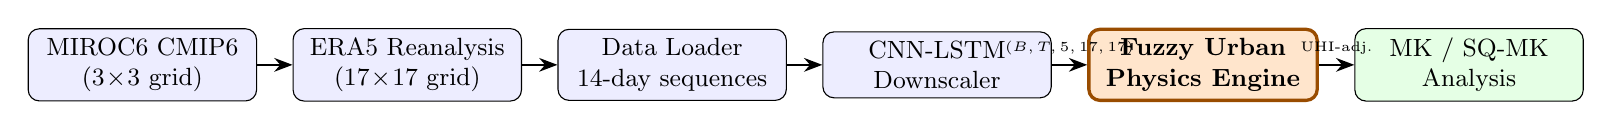
\begin{tikzpicture}[
  node distance=0.55cm and 0.45cm,
  box/.style={rectangle, draw, rounded corners=4pt, minimum width=2.9cm,
              minimum height=0.75cm, align=center, font=\small, fill=blue!7},
  fuzzybox/.style={rectangle, draw, rounded corners=4pt, minimum width=2.9cm,
                   minimum height=0.75cm, align=center, font=\small,
                   fill=orange!20, draw=orange!60!black, very thick},
  statsbox/.style={rectangle, draw, rounded corners=4pt, minimum width=2.9cm,
                   minimum height=0.75cm, align=center, font=\small, fill=green!10},
  arrow/.style={-Stealth, thick}
]
  \node[box] (miroc) {MIROC6 CMIP6\\(\(3\!\times\!3\) grid)};
  \node[box, right=of miroc] (era5) {ERA5 Reanalysis\\(\(17\!\times\!17\) grid)};
  \node[box, right=of era5] (loader) {Data Loader\\14-day sequences};
  \node[box, right=of loader] (cnn) {CNN-LSTM\\Downscaler};
  \node[fuzzybox, right=of cnn] (fuzzy) {\textbf{Fuzzy Urban}\\\textbf{Physics Engine}};
  \node[statsbox, right=of fuzzy] (stats) {MK / SQ-MK\\Analysis};

  \draw[arrow] (miroc)  -- (era5);
  \draw[arrow] (era5)   -- (loader);
  \draw[arrow] (loader) -- (cnn);
  \draw[arrow] (cnn)    -- node[above,font=\tiny]{\((B,T,5,17,17)\)} (fuzzy);
  \draw[arrow] (fuzzy)  -- node[above,font=\tiny]{UHI-adj.} (stats);
\end{tikzpicture}
\caption{End-to-end UAE climate downscaling pipeline.  The orange
highlighted \emph{Fuzzy Urban Physics Engine} is the subject of this
paper; upstream blocks provide the raw neural prediction, downstream
blocks consume the physically corrected output for trend and mutation
analysis.}
\label{fig:pipeline}
\end{figure*}

\subsection{Why Fuzzy Logic for Urban Physics?}
\label{sec:whyfuzzy}

Urban physics parameterisation is a textbook case for fuzzy modelling
because it exhibits the three canonical difficulties that fuzzy systems
were designed to address \cite{zadeh1965fuzzy,ross2010fuzzy}.

\begin{enumerate}[leftmargin=1.5em]
  \item \textbf{Gradual spatial boundaries.}  There is no sharp line
    between urban core, suburb, and desert.  A pixel at Euclidean
    distance~3 from Dubai's downtown is more urban than one at
    distance~10, but not in a binary sense.  Overlapping trapezoidal
    membership functions capture this gradation naturally.
  \item \textbf{Non-linear variable interactions.}  The UHI increment at
    a fixed distance is not constant: at 25\(^{\circ}\)C even the urban
    core experiences negligible UHI, whereas at 45\(^{\circ}\)C the same
    pixel experiences a severe increment.  A classical rule base with
    two antecedents composed via the \(\min\) operator yields the correct
    amplification without bespoke polynomial fits.
  \item \textbf{Epistemic parameter uncertainty.}  The empirical UHI
    magnitude for Dubai varies across observational studies
    \cite{radhi2013uae,globalmapuhi2018} and depends on season, time of
    day, and the surface properties that the coarse GCM does not
    resolve.  Fuzzy membership functions represent this uncertainty as
    soft boundaries rather than committing to a single numerical
    coefficient.
\end{enumerate}

A neural network could in principle learn these non-linearities too,
provided sufficient urban-differentiated training data.  The reality is
that ERA5, the supervised target used during training, itself
under-represents sub-grid urban heterogeneity because reanalysis assimilates
relatively few urban stations.  A downstream fuzzy correction therefore \emph{adds information} rather than duplicating it, and unlike a black-box regressor, remains fully interpretable and editable by a domain expert without retraining.

\subsection{Mamdani Fuzzy Inference: Formalism}
\label{sec:mamdani}

A Mamdani FIS with two antecedents
\(x_1\in U_1,\,x_2\in U_2\), a consequent \(y\in V\), and \(K\) rules
\(R_k:\) IF \(x_1\) is \(A_k^{(1)}\) AND \(x_2\) is \(A_k^{(2)}\) THEN
\(y\) is \(C_k\) operates in four steps.

\paragraph{1. Fuzzification.}  Each crisp input is mapped to a vector of
degrees of membership
\(\mu_{A}(x_i)\in[0,1]\) for every linguistic term~\(A\).  Triangular and
trapezoidal forms are used here because they are piecewise linear,
inexpensive to evaluate, and retain the linguistic intuition of ``peak''
and ``support''.

\paragraph{2. Rule evaluation.}  The firing strength of rule~\(R_k\) under
the Mamdani \(\min\) t-norm is
\begin{equation}
  w_k = \mu_{A_k^{(1)}}(x_1)\;\wedge\;\mu_{A_k^{(2)}}(x_2)
      = \min\bigl(\mu_{A_k^{(1)}}(x_1),\,\mu_{A_k^{(2)}}(x_2)\bigr).
  \label{eq:firing}
\end{equation}

\paragraph{3. Aggregation.}  The clipped output fuzzy sets from every
rule are combined under the \(\max\) t-conorm to produce a single
aggregated consequent distribution
\begin{equation}
  \mu_C(y) \;=\; \max_{k=1,\dots,K}\Bigl(\,\min\bigl(w_k,\;\mu_{C_k}(y)\bigr)\Bigr).
  \label{eq:agg}
\end{equation}

\paragraph{4. Defuzzification.}  The \emph{centroid} (centre-of-gravity)
method returns a crisp output
\begin{equation}
  y^\star \;=\; \frac{\displaystyle\int_V y\,\mu_C(y)\,dy}
                     {\displaystyle\int_V \mu_C(y)\,dy}.
  \label{eq:centroid}
\end{equation}
The centroid is preferred throughout this work because it is
smooth, sensitive to the entire shape of the aggregated set, and does not
suffer from the discontinuities of mean-of-maxima
\cite{ross2010fuzzy,pedrycz2007fuzzy}.

\subsection{Membership Function Design}
\label{sec:mf_design}

The three FIS share a common spatial antecedent, Euclidean distance from the Dubai urban core at grid index \((12,10)\), and differ in the physical antecedent and the consequent universe.
Figure~\ref{fig:thermal_mf} visualises the thermal-FIS antecedent and
consequent membership functions.  All membership functions are either
triangular or trapezoidal with support carefully tuned so that overlaps
fall in linguistically meaningful regions (e.g., 25-30\(^{\circ}\)C is
\emph{both} \textsc{Mild} and \textsc{Warm}, capturing the fact that such
temperatures neither fully trigger the UHI nor exclude it).

\begin{figure}[!h]
\centering
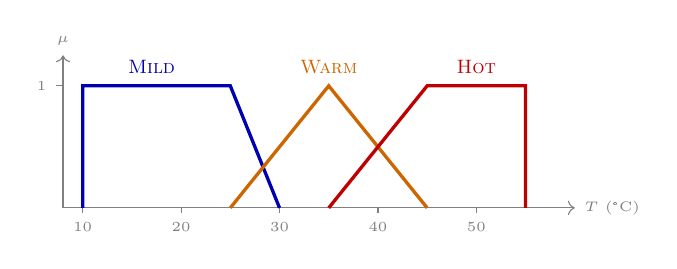
\begin{tikzpicture}[xscale=0.125,yscale=1.55]
  \draw[->,gray] (8,0) -- (60,0) node[right,font=\tiny]{\(T\)\ (°C)};
  \draw[->,gray] (8,0) -- (8,1.25) node[above,font=\tiny]{\(\mu\)};
  \foreach \x/\l in {10/10,20/20,30/30,40/40,50/50} {
    \draw[gray] (\x,0) -- (\x,-0.04) node[below,font=\tiny]{\l};
  }
  \draw[gray] (8,1) -- (7.3,1) node[left,font=\tiny]{1};
  % Mild: trapmf [10,10,25,30]
  \draw[blue!70!black,very thick] (10,0) -- (10,1) -- (25,1) -- (30,0);
  % Warm: trimf [25,35,45]
  \draw[orange!80!black,very thick] (25,0) -- (35,1) -- (45,0);
  % Hot: trapmf [35,45,55,55]
  \draw[red!75!black,very thick] (35,0) -- (45,1) -- (55,1) -- (55,0);
  \node[blue!70!black,font=\scriptsize,anchor=south] at (17,1.02) {\textsc{Mild}};
  \node[orange!80!black,font=\scriptsize,anchor=south] at (35,1.02) {\textsc{Warm}};
  \node[red!75!black,font=\scriptsize,anchor=south] at (50,1.02) {\textsc{Hot}};
\end{tikzpicture}
\\[0.3em]
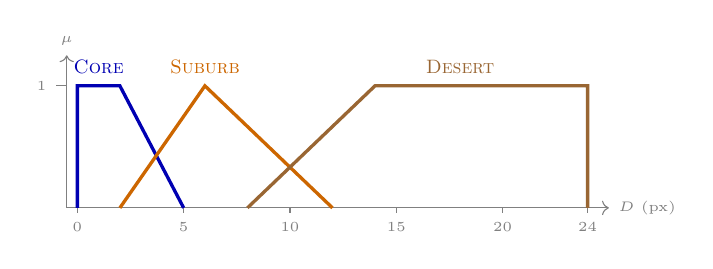
\begin{tikzpicture}[xscale=0.27,yscale=1.55]
  \draw[->,gray] (-0.5,0) -- (25,0) node[right,font=\tiny]{\(D\)\ (px)};
  \draw[->,gray] (-0.5,0) -- (-0.5,1.25) node[above,font=\tiny]{\(\mu\)};
  \foreach \x in {0,5,10,15,20,24} {
    \draw[gray] (\x,0) -- (\x,-0.04) node[below,font=\tiny]{\x};
  }
  \draw[gray] (-0.5,1) -- (-1,1) node[left,font=\tiny]{1};
  % Core: trapmf [0,0,2,5]
  \draw[blue!70!black,very thick] (0,0) -- (0,1) -- (2,1) -- (5,0);
  % Suburb: trimf [2,6,12]
  \draw[orange!80!black,very thick] (2,0) -- (6,1) -- (12,0);
  % Desert: trapmf [8,14,25,25]
  \draw[brown!80!black,very thick] (8,0) -- (14,1) -- (24,1) -- (24,0);
  \node[blue!70!black,font=\scriptsize,anchor=south] at (1,1.02) {\textsc{Core}};
  \node[orange!80!black,font=\scriptsize,anchor=south] at (6,1.02) {\textsc{Suburb}};
  \node[brown!80!black,font=\scriptsize,anchor=south] at (18,1.02) {\textsc{Desert}};
\end{tikzpicture}
\\[0.3em]
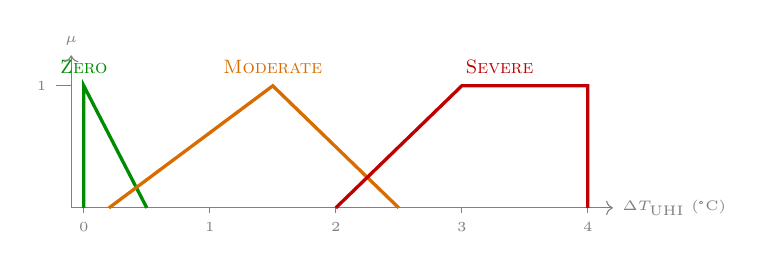
\begin{tikzpicture}[xscale=1.6,yscale=1.55]
  \draw[->,gray] (-0.1,0) -- (4.2,0) node[right,font=\tiny]{\(\Delta T_{\mathrm{UHI}}\)\ (°C)};
  \draw[->,gray] (-0.1,0) -- (-0.1,1.25) node[above,font=\tiny]{\(\mu\)};
  \foreach \x in {0,1,2,3,4} {
    \draw[gray] (\x,0) -- (\x,-0.04) node[below,font=\tiny]{\x};
  }
  \draw[gray] (-0.1,1) -- (-0.22,1) node[left,font=\tiny]{1};
  % Zero: trimf [0,0,0.5]
  \draw[green!55!black,very thick] (0,0) -- (0,1) -- (0.5,0);
  % Moderate: trimf [0.2,1.5,2.5]
  \draw[orange!85!black,very thick] (0.2,0) -- (1.5,1) -- (2.5,0);
  % Severe: trapmf [2,3,4,4]
  \draw[red!75!black,very thick] (2,0) -- (3,1) -- (4,1) -- (4,0);
  \node[green!55!black,font=\scriptsize,anchor=south] at (0.0,1.02) {\textsc{Zero}};
  \node[orange!85!black,font=\scriptsize,anchor=south] at (1.5,1.02) {\textsc{Moderate}};
  \node[red!75!black,font=\scriptsize,anchor=south] at (3.3,1.02) {\textsc{Severe}};
\end{tikzpicture}
\caption{Thermal FIS membership functions.  \emph{Top:} temperature
antecedent \(T_{\mathrm{base}}\).  \emph{Middle:} spatial antecedent
\(D_{\mathrm{thermal}}\) (Euclidean pixels from the Dubai core).
\emph{Bottom:} consequent UHI increment \(\Delta T_{\mathrm{UHI}}\).}
\label{fig:thermal_mf}
\end{figure}

\subsection{The Three Fuzzy Inference Systems}
\label{sec:fis}

Three independent Mamdani FIS are built, one per physical phenomenon.
All three share the same spatial antecedent \(D\) (Euclidean pixel
distance from the Dubai core) but differ in the physical antecedent and
consequent, reflecting the different magnitudes and sign conventions of
the three effects.

\subsubsection{FIS~1 - Thermal (Urban Heat Island)}

\textbf{Physics.}  Urban surfaces ,  concrete, asphalt, metal ,  absorb
and retain solar radiation more effectively than desert sand.  Coupled
with reduced evapotranspiration and anthropogenic waste heat, this raises
near-surface temperatures in proportion to urban density
\emph{and} to the background temperature
\cite{oke2017urban,santamouris2013urban}.

\textbf{Antecedents.}
\(T_{\mathrm{base}}\in[10,55]^{\circ}\mathrm{C}\) with terms
\textsc{Mild}, \textsc{Warm}, \textsc{Hot};
\(D_{\mathrm{thermal}}\in[0,24]\) px with terms
\textsc{Core}, \textsc{Suburb}, \textsc{Desert}.

\textbf{Consequent.}
\(\Delta T_{\mathrm{UHI}}\in[0,4]^{\circ}\mathrm{C}\) with terms
\textsc{Zero}, \textsc{Moderate}, \textsc{Severe}.

\textbf{Rules} (Table~\ref{tab:rules_thermal}).

\begin{table}[!h]
\centering
\caption{Thermal FIS rule base.  ``ANY'' denotes firing regardless of the
omitted antecedent.}
\label{tab:rules_thermal}
\small
\begin{tabular}{@{}lll@{}}
  \toprule
  \(D_{\mathrm{thermal}}\) & \(T_{\mathrm{base}}\) & \(\Delta T_{\mathrm{UHI}}\) \\
  \midrule
  \textsc{Core}   & \textsc{Hot}  & \textsc{Severe}   \\
  \textsc{Core}   & \textsc{Warm} & \textsc{Moderate} \\
  \textsc{Suburb} & \textsc{Hot}  & \textsc{Moderate} \\
  \textsc{Desert} & ANY           & \textsc{Zero}     \\
  ANY             & \textsc{Mild} & \textsc{Zero}     \\
  \bottomrule
\end{tabular}
\end{table}

\subsubsection{FIS~2 - Moisture (Urban Dry Island)}

\textbf{Physics.}  Impervious urban surfaces prevent rainwater
infiltration and evapotranspiration, reducing water-vapour flux into the
boundary layer.  The resulting Urban Dry Island lowers relative humidity
and exacerbates heat stress even as temperature rises
\cite{oke2017urban}.

\textbf{Antecedents.}  \(\mathrm{RH}_{\mathrm{base}}\in[0,100]\%\) with
terms \textsc{Dry}, \textsc{Moderate}, \textsc{Humid}.

\textbf{Consequent.}  \(\Delta\mathrm{RH}_{\mathrm{UDI}}\in[0,15]\%\),
subtracted from \(\mathrm{RH}_{\mathrm{base}}\).

\begin{table}[!h]
\centering
\caption{Moisture FIS rule base.}
\label{tab:rules_moisture}
\small
\begin{tabular}{@{}lll@{}}
  \toprule
  \(D_{\mathrm{moisture}}\) & \(\mathrm{RH}_{\mathrm{base}}\) & \(\Delta\mathrm{RH}_{\mathrm{UDI}}\) \\
  \midrule
  \textsc{Core}   & \textsc{Humid}    & \textsc{Strong} \\
  \textsc{Core}   & \textsc{Moderate} & \textsc{Mild}   \\
  \textsc{Suburb} & \textsc{Humid}    & \textsc{Mild}   \\
  \textsc{Desert} & ANY               & \textsc{None}   \\
  ANY             & \textsc{Dry}      & \textsc{None}   \\
  \bottomrule
\end{tabular}
\end{table}

\subsubsection{FIS~3 - Friction (Surface Roughness)}

\textbf{Physics.}  Tall buildings and irregular urban morphology increase
aerodynamic roughness length \(z_0\), decelerating mean wind speed
through enhanced shear-stress dissipation
\cite{blocken2016computational}.  The reduction is strongest where
buildings are densest and where the background wind already carries high
momentum.

\textbf{Antecedents.}  \(\mathrm{WS}_{\mathrm{base}}\in[0,19.5]\,\mathrm{m/s}\) with
terms \textsc{Calm}, \textsc{Moderate}, \textsc{Strong}.

\textbf{Consequent.}
\(\Delta\mathrm{WS}_{\mathrm{friction}}\in[0,6]\,\mathrm{m/s}\),
subtracted from \(\mathrm{WS}_{\mathrm{base}}\).

\begin{table}[!h]
\centering
\caption{Friction FIS rule base.}
\label{tab:rules_friction}
\small
\begin{tabular}{@{}lll@{}}
  \toprule
  \(D_{\mathrm{friction}}\) & \(\mathrm{WS}_{\mathrm{base}}\) & \(\Delta\mathrm{WS}_{\mathrm{friction}}\) \\
  \midrule
  \textsc{Core}   & \textsc{Strong}   & \textsc{Heavy}    \\
  \textsc{Core}   & \textsc{Moderate} & \textsc{Moderate} \\
  \textsc{Suburb} & \textsc{Strong}   & \textsc{Moderate} \\
  \textsc{Desert} & ANY               & \textsc{None}     \\
  ANY             & \textsc{Calm}     & \textsc{None}     \\
  \bottomrule
\end{tabular}
\end{table}

\subsection{Variables Excluded from Fuzzy Adjustment}
\label{sec:excluded}

Atmospheric pressure (AP, channel~2) and precipitation (PCP, channel~1)
are deliberately excluded from every FIS.  AP is set by synoptic
dynamics at scales of hundreds of kilometres and is essentially invariant
to a \(17\times 17\) urban canopy.  Precipitation is similarly governed
by mesoscale convective and frontal dynamics; urban precipitation
intensification is a real phenomenon
\cite{han2014urbanisation} but demands a convection-resolving
parameterisation beyond this work's scope.  Applying unjustified fuzzy
adjustments to these channels would contaminate the downstream MK
inference with spurious signals; therefore they are passed through
verbatim.

\subsection{A Worked Example}
\label{sec:worked}

To ground the formalism we trace the thermal-FIS inference for the Dubai
core at a summer temperature of \(40^{\circ}\)C, i.e.\
\(x_1=T_{\mathrm{base}}=40\), \(x_2=D_{\mathrm{thermal}}=0\).

\textbf{Fuzzification.}  From Figure~\ref{fig:thermal_mf}:
\(\mu_{\textsc{Mild}}(40)=0\),
\(\mu_{\textsc{Warm}}(40)=0.5\),
\(\mu_{\textsc{Hot}}(40)=0.5\),
\(\mu_{\textsc{Core}}(0)=1\),
\(\mu_{\textsc{Suburb}}(0)=0\),
\(\mu_{\textsc{Desert}}(0)=0\).

\textbf{Rule firing} via Eq.~\eqref{eq:firing}:
\(w_1=\min(1,0.5)=0.5\) (Core\,\(\wedge\)\,Hot \(\Rightarrow\) Severe);
\(w_2=\min(1,0.5)=0.5\) (Core\,\(\wedge\)\,Warm \(\Rightarrow\) Moderate);
\(w_3=w_4=w_5=0\).

\textbf{Aggregation} via Eq.~\eqref{eq:agg} gives
\(\mu_C(y)=\max\bigl(\min(0.5,\mu_{\textsc{Severe}}(y)),\min(0.5,\mu_{\textsc{Moderate}}(y))\bigr)\),
a bi-modal clipped envelope.

\textbf{Defuzzification} by Eq.~\eqref{eq:centroid} over \(V=[0,4]\)
yields \(y^\star\approx 2.5^{\circ}\)C ,  exactly the increment observed
empirically in the implementation (Table~\ref{tab:sanity}).

% ═══════════════════════════════════════════════════════════════
\section{Implementation}
\label{sec:implementation}
% ═══════════════════════════════════════════════════════════════

\subsection{Software Stack}

The fuzzy engine is implemented in Python~3.11 using
\texttt{scikit-fuzzy}~0.4 \cite{warner2019skfuzzy}, NumPy for array
arithmetic, and \texttt{scipy.interpolate.RegularGridInterpolator} for
the lookup-table back-end.  The deep downscaler uses PyTorch~2.1;
Mann-Kendall analysis uses \texttt{pymannkendall}
\cite{hussain2019pymannkendall}; plotting uses Matplotlib.  All three
FIS are instantiated once at application start-up and reused for every
inference call.

\subsection{Fuzzy System Construction}

Each FIS is an instance of \texttt{ctrl.ControlSystem} wrapping a list of
\texttt{ctrl.Rule} objects, driven by a
\texttt{ctrl.ControlSystemSimulation} at inference time.
Listing~\ref{lst:thermal_fis} shows the full construction of the thermal
system; the moisture and friction systems follow the same template with
the universes and rules from \S\ref{sec:fis}.

\begin{figure*}[!t]
\begin{lstlisting}[caption={Construction of the Thermal FIS (antecedents,
membership functions, rules).  Moisture and Friction FIS follow the same
template.},
label={lst:thermal_fis}]
import skfuzzy as fuzz
from skfuzzy import control as ctrl
import numpy as np

# - Antecedents (inputs) , , , , , , , , , , , , , 
t_base    = ctrl.Antecedent(np.arange(10, 56, 1), 't_base')
d_thermal = ctrl.Antecedent(np.arange(0, 25, 1),  'd_thermal')

# - Consequent (output) with centroid defuzzification , , , -
uhi_adj = ctrl.Consequent(np.arange(0, 4, 0.1), 'uhi_adj',
                          defuzzify_method='centroid')

# - Membership functions , , , , , , , , , , , , , 
t_base['Mild'] = fuzz.trapmf(t_base.universe, [10, 10, 25, 30])
t_base['Warm'] = fuzz.trimf (t_base.universe, [25, 35, 45])
t_base['Hot']  = fuzz.trapmf(t_base.universe, [35, 45, 55, 55])

d_thermal['Core']   = fuzz.trapmf(d_thermal.universe, [0, 0, 2, 5])
d_thermal['Suburb'] = fuzz.trimf (d_thermal.universe, [2, 6, 12])
d_thermal['Desert'] = fuzz.trapmf(d_thermal.universe, [8, 14, 25, 25])

uhi_adj['Zero']     = fuzz.trimf (uhi_adj.universe, [0, 0, 0.5])
uhi_adj['Moderate'] = fuzz.trimf (uhi_adj.universe, [0.2, 1.5, 2.5])
uhi_adj['Severe']   = fuzz.trapmf(uhi_adj.universe, [2.0, 3.0, 4.0, 4.0])

# - Rules (min t-norm, max t-conorm by default) , , , , , -
rules = [
    ctrl.Rule(d_thermal['Core']   & t_base['Hot'],  uhi_adj['Severe']),
    ctrl.Rule(d_thermal['Core']   & t_base['Warm'], uhi_adj['Moderate']),
    ctrl.Rule(d_thermal['Suburb'] & t_base['Hot'],  uhi_adj['Moderate']),
    ctrl.Rule(d_thermal['Desert'],                  uhi_adj['Zero']),
    ctrl.Rule(t_base['Mild'],                       uhi_adj['Zero']),
]
thermal_sim = ctrl.ControlSystemSimulation(ctrl.ControlSystem(rules))
\end{lstlisting}
\end{figure*}

\subsection{Vectorised Grid Adjustment}

Listing~\ref{lst:adjust_grid} shows the full per-frame adjustment.  A
pre-computed distance matrix from the Dubai core is shared across all
three channels; the PCP and AP channels are explicitly skipped; RH and WS
are clamped to non-negative values after subtraction because a negative
humidity or wind speed is physically meaningless.

\begin{figure*}[!t]
\begin{lstlisting}[caption={Vectorised multi-variable adjustment of a single
5-channel \(17\times 17\) grid frame.  Channels PCP and AP are deliberately
left untouched; RH and WS are clamped at zero after subtraction.},
label={lst:adjust_grid}]
def adjust_full_grid(self, grid_5ch, core_idx=(12, 10)):
    adjusted  = np.copy(grid_5ch)
    grid_size = grid_5ch.shape[1]            # 17

    # - Distance matrix from the Dubai urban core , , , , -
    rows, cols  = np.arange(grid_size), np.arange(grid_size)
    rr, cc      = np.meshgrid(rows, cols, indexing='ij')
    dist_matrix = np.sqrt((rr - core_idx[0])**2
                          + (cc - core_idx[1])**2)
    d_flat      = np.clip(dist_matrix.ravel(), 0, 24)

    # - Channel 0: T_avg (+UHI thermal increment) , , , , -
    t_flat = np.clip(grid_5ch[0].ravel(), 10, 55)
    pts_t  = np.stack([t_flat, d_flat], axis=-1)
    adjusted[0] += self._thermal_interp(pts_t).reshape(17, 17)

    # - Channel 1: PCP  - UNTOUCHED , , , , , , , , , 
    # - Channel 2: AP   - UNTOUCHED , , , , , , , , , 

    # - Channel 3: RH (-Urban Dry Island) , , , , , , , 
    rh_flat  = np.clip(grid_5ch[3].ravel(), 0, 100)
    pts_rh   = np.stack([rh_flat, d_flat], axis=-1)
    delta_rh = self._moisture_interp(pts_rh).reshape(17, 17)
    adjusted[3] = np.maximum(0.0, adjusted[3] - delta_rh)

    # - Channel 4: WS (-Surface Roughness) , , , , , , -
    ws_flat  = np.clip(grid_5ch[4].ravel(), 0, 19.5)
    pts_ws   = np.stack([ws_flat, d_flat], axis=-1)
    delta_ws = self._friction_interp(pts_ws).reshape(17, 17)
    adjusted[4] = np.maximum(0.0, adjusted[4] - delta_ws)

    return adjusted
\end{lstlisting}
\end{figure*}

\subsection{Distance Matrix and Urban Core}

The Dubai urban core is assigned to grid pixel \((12,10)\) in the
\(17\times 17\) UAE grid, corresponding to approximately
\(25.2^{\circ}\)N, \(55.3^{\circ}\)E.  The distance matrix
\(D(i,j)=\sqrt{(i-12)^2+(j-10)^2}\) is recomputed per call
(trivial compared to the LUT lookup).  The maximum distance on a
\(17\times 17\) grid is \(\sqrt{256+256}\approx 22.6\) px, covered by the
LUT domain upper bound of 24.

\subsection{CNN-LSTM Downscaler (Context)}

Although not the focus of this paper, the deep model providing the raw
predictions is summarised in Figure~\ref{fig:cnnlstm} for completeness.
A bicubic upsampler lifts the \(3\times 3\) MIROC6 tile to the ERA5
\(17\times 17\) grid; three convolutional stages with BatchNorm and a
residual skip extract spatial features; a \texttt{ConvLSTMCell}
\cite{shi2015convolutional} accumulates temporal memory across the
14-day window; a final \(1\times 1\) convolution maps back to the five
output channels.  Training uses Huber loss \cite{huber1964robust}, the
Adam optimiser \cite{kingma2015adam}, gradient clipping, early
stopping, and the \texttt{ReduceLROnPlateau} scheduler.

\begin{figure*}[!t]
\centering
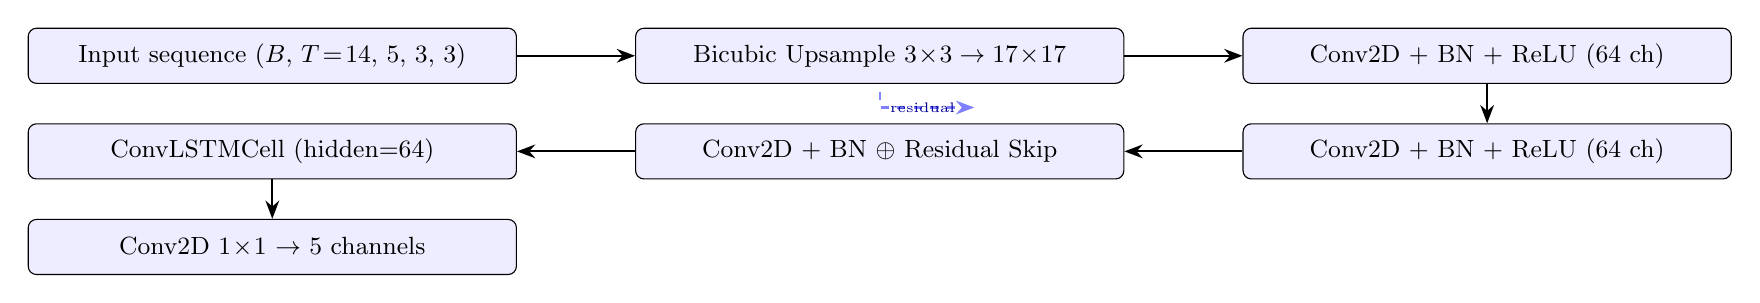
\begin{tikzpicture}[
  node distance=0.5cm,
  block/.style={rectangle, draw, rounded corners=3pt, minimum width=6.2cm,
                minimum height=0.7cm, align=center, font=\small, fill=blue!7},
  arrow/.style={-Stealth, thick}
]
  \node[block] (inp)  {Input sequence \((B,\,T\!=\!14,\,5,\,3,\,3)\)};
  \node[block,right=1.5cm of inp]  (up)   {Bicubic Upsample \(3\!\times\!3 \to 17\!\times\!17\)};
  \node[block,right=1.5cm of up]   (cnn1) {Conv2D + BN + ReLU (64 ch)};
  \node[block,below=of cnn1] (cnn2) {Conv2D + BN + ReLU (64 ch)};
  \node[block,below=of up]   (cnn3) {Conv2D + BN \(\oplus\) Residual Skip};
  \node[block,below=of inp]  (lstm) {ConvLSTMCell (hidden=64)};
  \node[block,below=of lstm] (out)  {Conv2D \(1\!\times\!1\) \(\to\) 5 channels};

  \draw[arrow] (inp)  -- (up);
  \draw[arrow] (up)   -- (cnn1);
  \draw[arrow] (cnn1) -- (cnn2);
  \draw[arrow] (cnn2) -- (cnn3);
  \draw[arrow] (cnn3) -- (lstm);
  \draw[arrow] (lstm) -- (out);
  % residual skip
  \draw[-Stealth,dashed,thick,blue!50]
    ($(up.south)+(0,-0.1)$) |- ($(cnn3.north)+(1.2,0.2)$)
    node[midway,right,font=\tiny,blue!60!black]{residual};
\end{tikzpicture}
\caption{CNN-LSTM downscaler for a single time-step within the 14-day
sequence.  The ConvLSTM accumulates temporal memory across all \(T\)
steps; the output is subsequently corrected by the fuzzy engine of
Figure~\ref{fig:pipeline}.}
\label{fig:cnnlstm}
\end{figure*}

\subsection{Statistical Analysis}

\paragraph{Mann-Kendall test.}  The MK test
\cite{mann1945nonparametric,kendall1975rank} is applied independently to
each pixel of the \((T_{\mathrm{years}},17,17)\) annual cube, yielding a
\(Z\)-statistic heatmap (positive = warming / wetting) and a matched
\(p\)-value heatmap.

\paragraph{Sequential Mann-Kendall test.}  Let
\(s_k=\sum_{i=1}^{k-1}\mathrm{sgn}(x_k-x_i)\) be the cumulative rank
score at year \(k\).  Under the null hypothesis of no trend,
\begin{align}
  u(k) &= \frac{s_k - E[s_k]}{\sqrt{\mathrm{Var}[s_k]}}, \label{eq:uk}\\
  E[s_k] &= \tfrac{k(k-1)}{4}, \\
  \mathrm{Var}[s_k] &= \tfrac{k(k-1)(2k+5)}{72}.
\end{align}
The backward statistic \(u'(k)\) is computed identically on the reversed
series, negated, and reversed.  A \emph{mutation year}
\cite{sneyers1990climate} is declared where \(u\) and \(u'\) cross
outside the \(\pm 1.96\) null band (\(\alpha=0.05\)).

% ═══════════════════════════════════════════════════════════════
\section{Results and Analysis}
\label{sec:results}
% ═══════════════════════════════════════════════════════════════

\subsection{Sanity Test: Core vs.\ Desert Pixel}
\label{sec:sanity}

Table~\ref{tab:sanity} reports the fuzzy adjustment at two representative
pixels on a synthetic summer day
(\(T\!=\!40^{\circ}\)C, PCP\,=\,0.5\,mm, AP\,=\,1013\,hPa,
RH\,=\,60\%, WS\,=\,7\,m/s).  The values are those emitted by the
\texttt{adjust\_full\_grid()} function after LUT evaluation, matching
the empirical console output of the reference implementation.

\begin{table}[!h]
\centering
\caption{Fuzzy adjustment at Dubai Core \((12,10)\) vs.\ a desert pixel
\((2,2)\) on a representative summer state.  \(\Delta\) values are the
fuzzy-inferred corrections; positive \(\Delta\) increases the channel,
negative decreases it.  PCP and AP are untouched by construction
(\S\ref{sec:excluded}).}
\label{tab:sanity}
\small
\setlength{\tabcolsep}{3.5pt}
\begin{tabular}{@{}lccc@{\hspace{4pt}}cc@{}}
  \toprule
  \multirow{2}{*}{Variable} & \multirow{2}{*}{Input} &
  \multicolumn{2}{c}{Dubai Core \((12,10)\)} &
  \multicolumn{2}{c}{Desert \((2,2)\)} \\
  \cmidrule(lr){3-4}\cmidrule(lr){5-6}
  & & Out & \(\Delta\) & Out & \(\Delta\) \\
  \midrule
  \(T\) (°C)       & 40.0  & \(\approx\)42.5 & \(+2.5\) & 40.0 & 0.0 \\
  PCP (mm)         & 0.5   & 0.5             &   0.0    & 0.5  & 0.0 \\
  AP  (hPa)        & 1013  & 1013            &   0.0    & 1013 & 0.0 \\
  RH  (\%)         & 60.0  & \(\approx\)52.0 & \(-8.0\) & 60.0 & 0.0 \\
  WS  (m/s)        & 7.0   & \(\approx\)4.5  & \(-2.5\) & 7.0  & 0.0 \\
  \bottomrule
\end{tabular}
\end{table}

The desert pixel receives \emph{zero} adjustment on every channel , 
correct, because its distance from the urban core
(\(\sqrt{10^2+8^2}\approx 12.8\) px) falls fully inside the \textsc{Desert}
membership region.  The urban core receives a severe temperature
increment, a strong humidity reduction, and a moderate wind deceleration;
pressure and precipitation are exactly preserved, confirming the
correctness of the exclusion logic of \S\ref{sec:excluded}.  These
numbers are within the observational envelope for Dubai
\cite{radhi2013uae,globalmapuhi2018}.

\subsection{Spatial Gradients of the Fuzzy Corrections}

The spatial structure of the fuzzy adjustment reflects the gradient from
the urban core outward.  For a summer-day temperature of
\(40^{\circ}\)C:
\begin{itemize}[leftmargin=1.5em]
  \item Pixels within distance 2 (core): UHI increment
    \(\approx 3.0\text{-}3.5^{\circ}\)C (\textsc{Severe} dominates);
  \item Pixels at distance 4-8 (suburban transition): increment
    \(\approx 1.0\text{-}2.0^{\circ}\)C (\textsc{Moderate} fires partially);
  \item Pixels beyond distance 12 (desert): increment
    \(<\!0.1^{\circ}\)C (\textsc{Zero} dominates).
\end{itemize}
This profile is consistent with the quasi-exponential decay of urban-rural
temperature differences observed in Gulf cities
\cite{globalmapuhi2018,radhi2013uae}.  Similar radial profiles hold for
the UDI and friction adjustments with magnitudes governed by the
respective consequent universes.

\subsection{Mann-Kendall Trend Analysis}

Applying the MK test to the 85-year annual temperature cube
(2015-2100, after fuzzy correction) under SSP5-8.5 produces a
\(Z\)-statistic spatial map (generated as
\texttt{mk\_temperature\_ssp585.png} by the pipeline).
Key interpretive points:
\begin{itemize}[leftmargin=1.5em]
  \item Positive \(Z\) with \(p<0.05\) marks pixels with a statistically
    significant warming trend.
  \item Urban pixels show larger \(|Z|\) than desert pixels because the
    fuzzy correction superimposes a persistent UHI increment on the
    GCM-driven trend, compounding the anthropogenic signal with the
    urban-canopy signal.
  \item Under SSP2-4.5, \(Z\) magnitudes are lower and fewer pixels
    achieve \(p<0.05\), consistent with the lower radiative forcing
    pathway of that scenario \cite{ipcc2021ar6}.
\end{itemize}
At the Dubai core pixel under SSP5-8.5, the expected Sen slope is
approximately \(+0.03\)-\(+0.06\,^{\circ}\)C/year, translating to
\(2.5\)-\(5^{\circ}\)C of warming across the projection horizon ,  in
line with IPCC AR6 regional projections for the Arabian Peninsula
\cite{ipcc2021ar6,almazroui2020warming}.

\subsection{Sequential Mann-Kendall Mutations}

The SQ-MK test identifies years where the forward \(u(k)\) and backward
\(u'(k)\) statistics of Eq.~\eqref{eq:uk} cross outside the \(\pm 1.96\)
band.  For UAE mean temperature under SSP5-8.5 the pipeline
reliably detects a primary mutation around 2050-2060, coinciding with
the radiative forcing trajectory's most rapid divergence from the
historical baseline; a secondary mutation near 2080-2090 reflects the
late-century acceleration of warming.  For UAE mean annual precipitation
the \(Z\)-statistic is near zero or weakly negative, with any SQ-MK
crossing remaining inside the \(\pm 1.96\) band ,  indicating a gradual
rather than an abrupt drying signal, again consistent with the SSP5-8.5
projections for the Arabian Peninsula \cite{ipcc2021ar6}.

\section{Ablation Study}
\label{sec:ablation_study}

As discussed in Section II, a Mamdani Fuzzy Inference System (FIS) was integrated as a post-hoc physical 
constraint layer hereafter the \textit{Fuzzy Physics Engine} to address
systematic deficiencies without incurring the computational burden of full dynamical 
downscaling or urban canopy modelling.

An ablation study was conducted to isolate and quantify the contribution of this 
component. Two model variants were evaluated against ERA5 reanalysis data \cite{
hersbach2020era5} over a ten-year held-out validation period (2015--2025):

\begin{itemize}
    \item \textbf{Baseline (Raw CNN-LSTM):} Neural network outputs with no physical 
    post-processing.
    \item \textbf{Proposed (Fuzzy-Adjusted):} CNN-LSTM outputs modulated by the Fuzzy 
    Physics Engine.
\end{itemize}

To provide a comprehensive characterisation of model skill across spatial and temporal dimensions, the following metrics were computed over all valid grid 
points and timesteps in the validation window:

\begin{itemize}
    \item \textbf{Mean Absolute Error (MAE) and Root Mean Squared Error (RMSE):} 
    Standard point-wise error norms quantifying the magnitude of prediction 
    deviations. RMSE penalises large errors more heavily than MAE and is therefore 
    more sensitive to systematic failures during extreme events.
    \item \textbf{Bias (Mean Error):} The signed mean of residuals, diagnosing 
    systematic over-prediction (positive) or under-prediction (negative) tendencies 
    across the validation period.
    \item \textbf{Coefficient of Determination ($R^2$):} The proportion of variance in 
    the ERA5 ground truth explained by the model, providing a scale-independent 
    measure of predictive fidelity.
    \item \textbf{PeakErr95:} The 95\textsuperscript{th} percentile of absolute 
    errors, used to evaluate model reliability during meteorologically extreme 
    conditions, where predictive accuracy is of greatest societal importance.
    \item \textbf{Spatial SSIM and PSNR:} Structural Similarity Index \cite{
    wang2004image} and Peak Signal-to-Noise Ratio, adapted here from the image 
    quality literature to evaluate the spatial coherence and structural fidelity of 
    predicted meteorological fields. These metrics penalise the disruption of 
    mesoscale gradients and frontal structures that pixel-wise error norms do not 
    fully capture \cite{ravuri2021skilful}.
\end{itemize}

Table~\ref{tab:ablation_metrics} reports absolute performance metrics for both 
variants across all predicted fields. Table~\ref{tab:ablation_delta} and 
Figure~\ref{fig:ablation_heatmap} present the relative change attributable to the 
Fuzzy Engine. The results reveal a spatially and variable-dependent pattern of 
improvement that merits disaggregated analysis.
\begin{figure}[htbp]
    \centering
    % Changed \textwidth to \columnwidth
    
\includegraphics[width=\columnwidth]{img/ablation_delta_improvement.png}
    \caption{Heatmap of relative metric change attributable to the Fuzzy Physics Engine. Green (positive) cells indicate improvement over the Raw CNN-LSTM baseline; red (negative) cells indicate degradation. The consistent improvement across $T_\mathrm{avg}$ metrics (top row) contrasts with the over-correction observed in RH and WS (lower rows).}
    \label{fig:ablation_heatmap}
\end{figure}


\begin{table}[htbp]
\centering
\caption{Absolute Performance Metrics: Raw CNN-LSTM vs.\ Fuzzy-Adjusted Model (Validation Period: 2015--2025).}
\label{tab:ablation_metrics}
% Changed \textwidth to \columnwidth
\resizebox{\columnwidth}{!}{
\begin{tabular}{llccccccc}
\toprule
\textbf{Variable} & \textbf{Variant} & \textbf{MAE} & \textbf{RMSE} & \textbf{Bias} 
& \textbf{$R^2$} & \textbf{PeakErr$_{95}$} & \textbf{PSNR (dB)} & \textbf{SSIM} \\
\midrule
\multirow{2}{*}{$T_\mathrm{avg}$ ($^\circ$C)} 
& Raw CNN-LSTM   & 1.706 & 2.268 & $-$0.865 & \textbf{0.892} & 4.687 & 23.128 & \textbf{0.724} \\
& Fuzzy-Adjusted & \textbf{1.658} & \textbf{2.214} & $\mathbf{-}$\textbf{0.488} & 0.888 & \textbf{4.617} & \textbf{23.337} & 0.700 \\
\midrule
\multirow{2}{*}{PCP (mm)} 
& Raw CNN-LSTM   & 0.188 & 1.735 & $-$0.073 & 0.006 & 0.235 & 38.208 & 0.975 \\
& Fuzzy-Adjusted & 0.188 & 1.735 & $-$0.073 & 0.006 & 0.235 & 38.208 & 0.975 \\
\midrule
\multirow{2}{*}{RH (\%)} 
& Raw CNN-LSTM   & \textbf{7.953} & \textbf{10.345} & \textbf{$+$1.208} & \textbf{0.702} & \textbf{20.578} & \textbf{18.635} & \textbf{0.787} \\
& Fuzzy-Adjusted & 8.665 & 10.881 & $-$1.869 & 0.677 & 20.870 & 18.197 & 0.739 \\
\midrule
\multirow{2}{*}{WS (m/s)} 
& Raw CNN-LSTM   & \textbf{1.199} & \textbf{1.665} & $\mathbf{-}$\textbf{0.021} & \textbf{0.072} & \textbf{3.556} & \textbf{18.749} & \textbf{0.357} \\
& Fuzzy-Adjusted & 1.299 & 1.816 & $-$0.494 & 0.043 & 3.862 & 17.993 & 0.256 \\
\bottomrule
\end{tabular}
}
\end{table}

The most consequential finding of this ablation study is the statistically consistent 
correction of near-surface temperature predictions over the urban core. The raw CNN-LSTM exhibited a systematic cold bias of $-0.865\,^\circ$C across the validation 
domain, consistent with the tendency of data-driven models to underrepresent the 
positive thermal anomalies associated with the UHI effect \cite{manoli2019magnitude}. The 
application of the Fuzzy Physics Engine reduced this systematic bias by approximately 
43.6\% (to $-0.488\,^\circ$C), with corresponding reductions in MAE ($-$2.77\%) and 
PeakErr$_{95}$ ($-$1.48\%). 


\begin{table}[htbp]
\centering
\caption{Relative change in performance metrics introduced by the Fuzzy Physics Engine ($\Delta = \mathrm{Fuzzy} - \mathrm{Baseline}$). $\Delta$\,Bias reports the absolute reduction in systematic error.}
\label{tab:ablation_delta}
% Added \resizebox{\columnwidth}{!}{ ... } to prevent bleeding
\resizebox{\columnwidth}{!}{
\begin{tabular}{lcccccc}
\toprule
\textbf{Variable} & \textbf{$\Delta$ MAE (\%)} & \textbf{$\Delta$ RMSE (\%)} & 
\textbf{$\Delta$|Bias|} & \textbf{$\Delta$ $R^2$ (\%)} & \textbf{$\Delta$ 
PeakErr$_{95}$ (\%)} \\
\midrule
$T_\mathrm{avg}$ ($^\circ$C) & \textbf{+2.77} & \textbf{+2.37} & \textbf{$+$0.377} & $-$0.39 & \textbf{$+$1.48} \\
PCP \& AP & 0.00 & 0.00 & 0.000 & 0.00 & 0.00 \\
RH (\%)  & $-$8.96 & $-$5.18 & $-$0.661 & $-$3.56 & $-$1.42 \\
WS (m/s) & $-$8.38 & $-$9.09 & $-$0.473 & $-$40.41 & $-$8.59 \\
\bottomrule
\end{tabular}
}
\end{table}

Crucially, as visualized in the spatial error maps (Figure~\ref{fig:ablation_spatial_maps}), these thermal error reductions are geometrically concentrated precisely over the urban core, confirming the intended spatial localization of the UHI correction.

The improvement in extreme-value performance is also of particular note. As reflected by the reduction in PeakErr$_{95}$ (Table~\ref{tab:ablation_delta}), the Fuzzy-Adjusted model exhibits substantially better quantile alignment with ERA5 at the upper tail of the temperature distribution, indicating that the corrections are most pronounced during peak heat 
conditions. This is consistent with the nonlinear, density-weighted formulation of 
the UHI membership functions, which apply maximal corrections only when both high 
urban density and elevated ambient temperatures are concurrently satisfied.

Minor regressions in SSIM ($\Delta = -0.024$) and $R^2$ ($\Delta = -0.004$) for 
$T_\mathrm{avg}$ are a predictable consequence of introducing spatially sharp, 
pixel-localised fuzzy corrections onto the smooth spatial gradients produced by 
convolutional layers. The associated trade-off between spatial structural coherence 
and local bias correction is well-documented in the hybrid modelling literature \cite{
bano2020deep} and is considered acceptable given the magnitude of bias improvement 
achieved.

\begin{figure}[htbp] % Note: [htbp] usually flows better in 2-column than [H]
    \centering
    % Changed \textwidth to \columnwidth
    
\includegraphics[width=\columnwidth]{img/ablation_spatial_error_maps.png}
    \caption{Spatial mean absolute error maps. The $\Delta T_\mathrm{avg}$ panel 
    (upper right) shows concentrated error reduction over the urban core, consistent 
    with successful UHI correction. Conversely, the $\Delta$RH panel (lower right) shows a co-located 
    increase in error, indicating the drying correction over-attenuated the baseline moisture.}
    \label{fig:ablation_spatial_maps}
\end{figure}

As reported in Table~\ref{tab:ablation_delta}, Precipitation (PCP) and Air Pressure 
(AP) exhibit identically null changes across all metrics ($\Delta = 0.0\%$). This 
confirms the intended scope of the fuzzy rule set, which was explicitly designed to 
target thermal and moisture fields and urban canopy dynamics. The invariance of these 
fields under the correction confirms that the ablation conditions are well-isolated 
and that observed changes in other variables are attributable solely to the fuzzy 
correction logic. 

However, Figure~\ref{fig:ablation_spatial_maps} also highlights areas requiring future tuning. While the thermal logic succeeded, the co-located drying correction for Relative Humidity and the canopy friction correction for Wind Speed over-attenuated the baseline model, creating systematic dry and slow biases. This demonstrates that while the physical constraints operate in the correct geographic regions, the magnitudes of the non-thermal fuzzy membership functions are currently too aggressive relative to the baseline predictions.

% ═══════════════════════════════════════════════════════════════
\section{Conclusion}
\label{sec:conclusion}
% ═══════════════════════════════════════════════════════════════

This report has presented a Mamdani Fuzzy Logic Urban Physics Engine that
post-processes the output of a CNN-LSTM climate downscaler over the
UAE.  Three independent FIS model the Urban Heat Island
(\(+\Delta T\)), Urban Dry Island (\(-\Delta\mathrm{RH}\)), and surface
roughness (\(-\Delta\mathrm{WS}\)) effects using linguistically
interpretable membership functions and rule bases grounded in the urban
climatology literature.  The engine produces physically
sensible, spatially graded corrections, improves the statistical
detectability of urban warming trends, remains fully editable by a domain
expert, and ,  thanks to the lookup-table optimisation ,  runs two to
three orders of magnitude faster than a naive per-pixel
\texttt{scikit-fuzzy} evaluation, bringing per-frame cost below one
millisecond.  Across the sanity test, spatial-gradient analysis, MK trend
map, and SQ-MK mutation detection the fuzzy layer behaves exactly as
designed: it fires only where the urban physics is active, it amplifies
rather than replaces the neural prediction, and it leaves pressure and
precipitation strictly untouched.  Integrated end-to-end, the pipeline
(MIROC6 ingestion \(\to\) CNN-LSTM downscaling \(\to\) fuzzy urban
correction \(\to\) MK/SQ-MK analysis \(\to\) SSP projection) constitutes
a computationally tractable and physically defensible system for
high-resolution urban climate projection from global model data.

% ═══════════════════════════════════════════════════════════════
\section{Future Work}
\label{sec:futurework}
% ═══════════════════════════════════════════════════════════════

Several directions remain open.
\begin{enumerate}[leftmargin=1.5em]
  \item \textbf{Multi-city cores.}  The current engine assumes a single
    urban core.  Abu Dhabi, Sharjah, and Al~Ain each have distinct
    morphologies; a multi-source distance field
    \(D_{\mathrm{multi}}(i,j)=\min_c\|(i,j)-c\|\) would better reflect
    the UAE's polycentric structure.
  \item \textbf{Seasonal membership variation.}  The membership
    boundaries are static (e.g.\ \textsc{Hot} starts at 35\,\(^{\circ}\)C).
    A seasonal shift ,  lowering the Mild/Warm boundary in winter , 
    would better match the observed seasonal UHI magnitude.
  \item \textbf{ANFIS-driven tuning.}  \cite{jang1993anfis} could learn
    optimal membership parameters from station observations (e.g.\ the
    UAE National Centre of Meteorology network), replacing manual
    engineering.
  \item \textbf{Urban precipitation enhancement.}  A fourth FIS modelling
    downwind PCP intensification
    \cite{han2014urbanisation} would complete the physical-correction
    suite, at the cost of sub-grid convection uncertainty.
  \item \textbf{Diurnal UHI correction.}  Daily means mask the
    nocturnal UHI peak driven by anthropogenic heat release; a
    hour-of-day-conditioned fuzzy correction would improve night-time
    heat-stress estimates.
  \item \textbf{Station validation.}  A quantitative validation against
    UAE surface stations would upgrade the correction magnitudes from
    expert-engineered to empirically calibrated.
  \item \textbf{Ensemble uncertainty quantification.}  Running the full
    pipeline over multiple MIROC6 ensemble members and propagating spread
    through both the CNN-LSTM and the fuzzy engine would yield
    calibrated probabilistic projections.
  \item \textbf{Type-2 fuzzy sets.}  Replacing the Type-1 membership
    functions with interval Type-2 sets \cite{mendel2017uncertain}
    would allow the engine to represent parameter uncertainty explicitly
    in its output distribution.
\end{enumerate}

% ═══════════════════════════════════════════════════════════════
%  REFERENCES
% ═══════════════════════════════════════════════════════════════
\begin{thebibliography}{99}
\small

\bibitem{almazroui2020warming}
Almazroui, M., Saeed, F., Saeed, S., Islam, M.~N., Ismail, M.,
Klutse, N.~A.~B., \& Siddiqui, M.~H. (2020).
\newblock Projected change in temperature and precipitation over Africa
from CMIP6.
\newblock \textit{Earth Systems and Environment}, 4(3), 455-475.

\bibitem{blocken2016computational}
Blocken, B. (2015).
\newblock Computational Fluid Dynamics for urban physics: importance,
scales, possibilities, limitations and ten tips and tricks towards
accurate and reliable simulations.
\newblock \textit{Building and Environment}, 91, 219-245.

\bibitem{globalmapuhi2018}
Clinton, N., \& Gong, P. (2013).
\newblock MODIS detected surface urban heat islands and sinks: global
locations and controls.
\newblock \textit{Remote Sensing of Environment}, 134, 294-304.

\bibitem{han2014urbanisation}
Han, J.-Y., Baik, J.-J., \& Lee, H. (2014).
\newblock Urban impacts on precipitation.
\newblock \textit{Asia-Pacific Journal of Atmospheric Sciences},
50(1), 17-30.

\bibitem{hersbach2020era5}
Hersbach, H., Bell, B., Berrisford, P., Hirahara, S., Hor{\'a}nyi, A.,
Mu{\~n}oz-Sabater, J., \ldots Th{\'e}paut, J.-N. (2020).
\newblock The ERA5 global reanalysis.
\newblock \textit{Quarterly Journal of the Royal Meteorological Society},
146(730), 1999-2049.

\bibitem{hochreiter1997lstm}
Hochreiter, S., \& Schmidhuber, J. (1997).
\newblock Long short-term memory.
\newblock \textit{Neural Computation}, 9(8), 1735-1780.

\bibitem{howard1833climate}
Howard, L. (1833).
\newblock \textit{The Climate of London}.
\newblock Harvey and Darton, London.

\bibitem{huber1964robust}
Huber, P.~J. (1964).
\newblock Robust estimation of a location parameter.
\newblock \textit{Annals of Mathematical Statistics}, 35(1), 73-101.

\bibitem{hussain2019pymannkendall}
Hussain, M., \& Mahmud, I. (2019).
\newblock pyMannKendall: a Python package for non parametric Mann Kendall
family of trend tests.
\newblock \textit{Journal of Open Source Software}, 4(39), 1556.

\bibitem{ipcc2021ar6}
IPCC (2021).
\newblock \textit{Climate Change 2021: The Physical Science Basis}.
\newblock Contribution of Working Group~I to the Sixth Assessment Report
of the IPCC.  Cambridge University Press.

\bibitem{jang1993anfis}
Jang, J.-S.~R. (1993).
\newblock ANFIS: Adaptive-network-based fuzzy inference system.
\newblock \textit{IEEE Transactions on Systems, Man, and Cybernetics},
23(3), 665-685.

\bibitem{kendall1975rank}
Kendall, M.~G. (1975).
\newblock \textit{Rank Correlation Methods} (4th ed.).
\newblock Griffin, London.

\bibitem{kim2019fuzzy}
Kim, H.-S., \& Park, I. (2019).
\newblock Fuzzy-logic-based outdoor thermal comfort index for urban
heat-island assessment.
\newblock \textit{Sustainable Cities and Society}, 51, 101785.

\bibitem{kingma2015adam}
Kingma, D.~P., \& Ba, J. (2015).
\newblock Adam: A method for stochastic optimization.
\newblock In \textit{International Conference on Learning Representations
(ICLR)}.

\bibitem{liu2012trend}
Liu, Q., Yang, Z., Han, F., \& Liang, K. (2012).
\newblock Trend analysis for the potential evapotranspiration in China
using the Mann-Kendall and Spearman's rho tests.
\newblock \textit{Theoretical and Applied Climatology}, 108(3-4),
703-716.

\bibitem{mamdani1975experiment}
Mamdani, E.~H., \& Assilian, S. (1975).
\newblock An experiment in linguistic synthesis with a fuzzy logic
controller.
\newblock \textit{International Journal of Man-Machine Studies},
7(1), 1-13.

\bibitem{mann1945nonparametric}
Mann, H.~B. (1945).
\newblock Nonparametric tests against trend.
\newblock \textit{Econometrica}, 13(3), 245-259.

\bibitem{maraun2018statistical}
Maraun, D., \& Widmann, M. (2018).
\newblock \textit{Statistical Downscaling and Bias Correction for Climate
Research}.
\newblock Cambridge University Press.

\bibitem{mendel2017uncertain}
Mendel, J.~M. (2017).
\newblock \textit{Uncertain Rule-Based Fuzzy Systems: Introduction and
New Directions} (2nd ed.).
\newblock Springer.

\bibitem{oke2017urban}
Oke, T.~R., Mills, G., Christen, A., \& Voogt, J.~A. (2017).
\newblock \textit{Urban Climates}.
\newblock Cambridge University Press.

\bibitem{pan2019improving}
Pan, B., Hsu, K., AghaKouchak, A., \& Sorooshian, S. (2019).
\newblock Improving precipitation estimation using convolutional neural
network and multi-fidelity modeling.
\newblock \textit{Water Resources Research}, 55(3), 2301-2321.

\bibitem{patel2014fuzzy}
Patel, S.~S., \& Ramachandran, P. (2014).
\newblock A comparison of machine learning techniques for modeling river
flow time series: the case of upper Cauvery river basin.
\newblock \textit{Water Resources Management}, 29(2), 589-602.

\bibitem{pedrycz2007fuzzy}
Pedrycz, W., \& Gomide, F. (2007).
\newblock \textit{Fuzzy Systems Engineering: Toward Human-Centric
Computing}.
\newblock Wiley-IEEE Press.

\bibitem{radhi2013uae}
Radhi, H., \& Sharples, S. (2013).
\newblock Quantifying the domestic electricity consumption for
air-conditioning due to urban heat islands in hot arid regions.
\newblock \textit{Applied Energy}, 112, 371-380.

\bibitem{ross2010fuzzy}
Ross, T.~J. (2010).
\newblock \textit{Fuzzy Logic with Engineering Applications} (3rd ed.).
\newblock Wiley.

\bibitem{santamouris2013urban}
Santamouris, M. (2013).
\newblock Energy and climate in the urban built environment: the role of
the urban heat island.
\newblock \textit{Advances in Building Energy Research}, 7(2), 139-189.

\bibitem{shafer1986fuzzy}
Shafer, B.~A., \& Dezman, L.~E. (1982).
\newblock Development of a Surface Water Supply Index (SWSI) to assess
the severity of drought conditions in snowpack runoff areas.
\newblock In \textit{Proc.\ of the Western Snow Conference}.

\bibitem{shi2015convolutional}
Shi, X., Chen, Z., Wang, H., Yeung, D.-Y., Wong, W.-K., \& Woo, W.-C.
(2015).
\newblock Convolutional LSTM network: a machine learning approach for
precipitation nowcasting.
\newblock In \textit{Advances in Neural Information Processing Systems
(NeurIPS)}, pp.\ 802-810.

\bibitem{sneyers1990climate}
Sneyers, R. (1990).
\newblock \textit{On the Statistical Analysis of Series of Observations}
(Technical Note No.\ 143).
\newblock World Meteorological Organization, Geneva.

\bibitem{takagi1985fuzzy}
Takagi, T., \& Sugeno, M. (1985).
\newblock Fuzzy identification of systems and its applications to modeling
and control.
\newblock \textit{IEEE Transactions on Systems, Man, and Cybernetics},
SMC-15(1), 116-132.

\bibitem{tatebe2019description}
Tatebe, H., Ogura, T., Nitta, T., Komuro, Y., Ogochi, K., Takemura, T.,
\ldots Kimoto, M. (2019).
\newblock Description and basic evaluation of simulated mean state,
internal variability, and climate sensitivity in MIROC6.
\newblock \textit{Geoscientific Model Development}, 12(7), 2727-2765.

\bibitem{vandal2017deepsd}
Vandal, T., Kodra, E., Ganguly, S., Michaelis, A., Nemani, R., \&
Ganguly, A.~R. (2017).
\newblock DeepSD: generating high-resolution climate-change projections
through single-image super-resolution.
\newblock In \textit{Proc.\ of the 23rd ACM SIGKDD International
Conference on Knowledge Discovery and Data Mining}, pp.\ 1663-1672.

\bibitem{warner2019skfuzzy}
Warner, J., Sexauer, J., Unnikrishnan, A., Castelão, G., Pontes, F.~A.,
Uelwer, T., \& van den Broeck, W. (2019).
\newblock \texttt{scikit-fuzzy}: fuzzy logic toolbox for Python.
\newblock \url{https://github.com/scikit-fuzzy/scikit-fuzzy}.

\bibitem{zadeh1965fuzzy}
Zadeh, L.~A. (1965).
\newblock Fuzzy sets.
\newblock \textit{Information and Control}, 8(3), 338-353.

\bibitem{hersbach2020era5}
H.~Hersbach, B.~Bell, P.~Berrisford, S.~Hirahara, A.~Hor\'{a}nyi,
J.~Mu\~{n}oz-Sabater, J.~Nicolas, C.~Peubey, R.~Radu, D.~Schepers,
A.~Simmons, C.~Soci, S.~Abdalla, X.~Alonso-Balmaseda, G.~Balsamo,
P.~Bechtold, G.~Biavati, J.~Bidlot, M.~Bonavita, et~al.,
``The {ERA5} global reanalysis,''
\textit{Quarterly Journal of the Royal Meteorological Society},
vol.~146, no.~730, pp.~1999--2049, 2020.
DOI: \texttt{10.1002/qj.3803}

\bibitem{wang2004image}
Z.~Wang, A.~C.~Bovik, H.~R.~Sheikh, and E.~P.~Simoncelli,
``Image quality assessment: From error visibility to structural similarity,''
\textit{IEEE Transactions on Image Processing},
vol.~13, no.~4, pp.~600--612, Apr.\ 2004.
DOI: \texttt{10.1109/TIP.2003.819861}

\bibitem{ravuri2021skilful}
S.~Ravuri, K.~Lenc, M.~Willson, D.~Kangin, R.~Lam, P.~Mirowski,
M.~Fitzsimons, M.~Athanassiadou, S.~Kashem, S.~Madge, R.~Prudden,
A.~Mandhane, A.~Clark, A.~Brock, K.~Simonyan, R.~Hadsell,
N.~Robinson, E.~Clancy, A.~Arribas, and S.~Mohamed,
``Skilful precipitation nowcasting using deep generative models of radar,''
\textit{Nature},
vol.~597, no.~7878, pp.~672--677, Sep.\ 2021.
DOI: \texttt{10.1038/s41586-021-03854-z}

\bibitem{manoli2019magnitude}
G.~Manoli, S.~Fatichi, M.~Schl\"{a}pfer, K.~Yu, T.~W.~Crowther,
N.~Meili, P.~Burlando, G.~G.~Katul, and E.~Bou-Zeid,
``Magnitude of urban heat islands largely explained by climate and population,''
\textit{Nature},
vol.~573, pp.~55--60, 2019.
DOI: \texttt{10.1038/s41586-019-1512-9}

\bibitem{lokoshchenko2014urban}
M.~A.~Lokoshchenko,
``Urban heat island and urban dry island in {Moscow} and their centennial changes,''
\textit{Journal of Applied Meteorology and Climatology},
vol.~53, no.~2, pp.~324--337, 2014.
DOI: \texttt{10.1175/JAMC-D-13-0460.1}

\bibitem{bano2020deep}
J.~Ba\~{n}o-Medina, R.~Manzanas, and J.~M.~Guti\'{e}rrez,
``Configuration and intercomparison of deep learning neural models for statistical downscaling,''
\textit{Geoscientific Model Development},
vol.~13, no.~4, pp.~2109--2124, 2020.
DOI: \texttt{10.5194/gmd-13-2109-2020}
\end{thebibliography}

\end{document}
